\chapter{History Reuse Architecture}
\label{chap-four}

\section{Overview}
\label{overview}
For any framework to be successful globally in the computation of History Reuse needed to effectively and comprehensively solve all the challenges motioned above. In addition it also needed to be directly translatable and not be over dependent upon the algorithm in question. Keeping the above framework requirements in mind we finally settle on the framework components as follows:
\subsection{Feature Set Reduction And Normalization}
\label{fet_set_red}
The aim of this section of the framework is to capture the most relevant features of the data set (features along which maximum variation is seen). For this purpose we decided to take a leaf out of the Image processing/statistics books. This step consists of two major parts:
\begin{itemize}
    \item \textbf{Dimension Reduction:} In this part of the algorithm we essentially reduce the total dimensions of the data set to the minimal possible without losing the meaning of the data set. This is achieved by the use of Principal Component Analysis (PCA)\cite{pca}\cite{pca_visual}. PCA is a method, which takes in a data set, and then proceeds to return a modified data set such that the dimensions in the updated normalized data set are arranged in descending order of variance. This way we can take the top few dimensions for our computations.
    \item \textbf{Point Count Reduction:} In this part of the algorithm we essentially aim at selecting the optimal sample set of data-points from the data set for our computations. This is essentially achieved by dividing all the points into buckets. We then proceed to pick the top-k highest populated buckets to get the highest density range of the data set, while at the same time greatly reducing the total no of data-points that needing consideration in our data set.
\end{itemize}
\subsection{Similarity Metric Calculation}
\label{sim_calc}
\begin{itemize}
    \item Once we have evaluated the reduced data-set using steps mentioned in section 5.1, we proceed to calculate the probability based similarity metric. We achieve this using \textbf{\textit{Welch’s Test}}\cite{welch_test} for non-parameterized data for null hypothesis testing. In statistics, Welch's t-test (or unequal variances t-test) is a two-sample location test, and is used to test the hypothesis that two populations have equal means. Welch's t-test is an adaptation of Student's t-test, and is more reliable when the two samples have unequal variances and unequal sample sizes. In our algorithm, we use it to approximate the degree of similarity of means between our current data set and our historic data sets. 
    \item Our assumed null hypothesis for any compared data sets is that both data sets are exactly similar to each other. The Welch test thus gives us a probability metric that states that the difference in data sets is due to chance based on the evaluation of the difference in their means. Thus higher the probability of the difference in data sets being up to chance, the better is the probability that the two sets would be similar. We choose the Welch's test because it gives more accurate results as compared to the Student T-Test for data sets whose distribution in non-Gaussian and whose sample size may be different.
    \item We take individual dimensions from the two data-sets and run Welch Test on them to get a probabilistic measure of their similarity on a per dimension and a cumulative sum across dimensions. We then rank the data sets with respect to each other based on the computed probabilistic metrics. Now this is an important aspect of our computation because this is the algorithm that we used for our probabilistic metric calculation, which is in turn used for ranking all data sets relative to each other.
\end{itemize}
\subsection{History Storage Architecture}
Once we have computed the above-mentioned values for our data set, we store it in memory as objects. Each historical data object holds its original data, PCA metadata (Eigen values and Eigen vectors etc.), bucket-wise histogram and the reduced data set. In addition to this each object also stores a score of the probabilistic similarity it holds with each of the other historical data sets and maintains them in non-increasing order of probability. This is done for quick access of data sets for computations when we are comparing real-time data with historical data sets.
\subsection{Matcher and Selector}
This is by far the most time critical part of the framework. It needs to be quick because this is the function that is responsible for matching the current data set with the sets in the historical data-set and find the best match for computation reuse selection in real-time. Since, historical data may be large, we need a quick way to find the closest match from the historical data set. Our framework goes about doing this in the following two passes:
\begin{itemize}
    \item In the first pass we do the PCA computation for our current set. We then proceed to use the histogram made by the PCA data points for quick distance comparison. We take the highest populated top-k buckets and do a distance computation with points in similar buckets in other data sets. This gives us one candidate for History Reuse. Another candidate is calculated by computing distance as mentioned above but in this case instead of taking highest populated buckets from History Reuse candidates, we now use buckets having closest ranges to the selected buckets for current data set. This is done to estimate similarity in distribution. Doing this we now get another candidate for history reuse. This part of the algorithm runs linearly without much time delay. Thus we can afford to do this kind of matching with all the historical data sets and get the approximate closest match.
    
    \item We now use the above computed candidate historical data sets along with the current data set to compute the probabilistic metric of similarity between the data sets and then proceed to compute the same metric for the top three closest matches to the historical data sets (pre-computed and stored.) We now use the data set with the highest probabilistic similarity to select data set for computation reuse. This step gives us the final candidate for History Reuse.
\end{itemize}

\section{Algorithm: HRu Architecture}
The final algorithm maybe divided into two major categories: Training and Run Time. 
\begin{itemize}
	\item \textbf{Training Algorithm}: The training algorithm is used to prepare and store data so as to have highest availability of reuse components for all candidates. This part of the algorithm is carried out offline and thus does not affect the run time of the algorithm when run for most current data set.
	\item \textbf{Run Time Algorithm:} The run time algorithm is responsible for choosing the best match historical data set to be used for Computation Reuse. This part of the algorithm is online, thus it has a direct impact on the run time for the algorithm when run for current data set. This part of the algorithm must be quick and must ensure that the computation time required for historical data set selection not overshoot the time for benefits gained by such history reuse.
\end{itemize}

Both the training algorithm and the run time algorithm use some complex methodologies to ensure the best possible approach for historical data set selection. These are defined in the following sub sections.

\subsection{Principal Component Analysis (PCA)}
\label{principal_comp_analysis}
	PCA\cite{pca}\cite{opencv_library} \cite{opencv_manual} and project data set points on thus computed Eigen vectors. PCA essentially extracts the top \textit{n} most influential \textit{features} of a data set. For our algorithm we choose the \textbf{top 3 principal components.} PCA returns Eigen vectors for the three chosen principal axis (or components) for our data set based on maximum variance for each feature set (represented by a single column). We then proceed to project the data onto the new Eigen plane using the above computed Eigen vectors. This step reduces the dimensionality of our data into a fixed three-dimension space.
\textbf{figure}  \ref{subfig:pca_real_data} shows an example data distribution in a 2-D plane and \textbf{figure} \ref{subfig:pca_proj_data} shows the same data projected into a 2-D Eigen plane. Since Eigen planes are always coplanar, this thus normalizes the data along the same axes. 

\begin{figure}[!ht]
	\centering
    \subfloat[Example: Real Data with 2 Dimensions\label{subfig:pca_real_data}]{%
      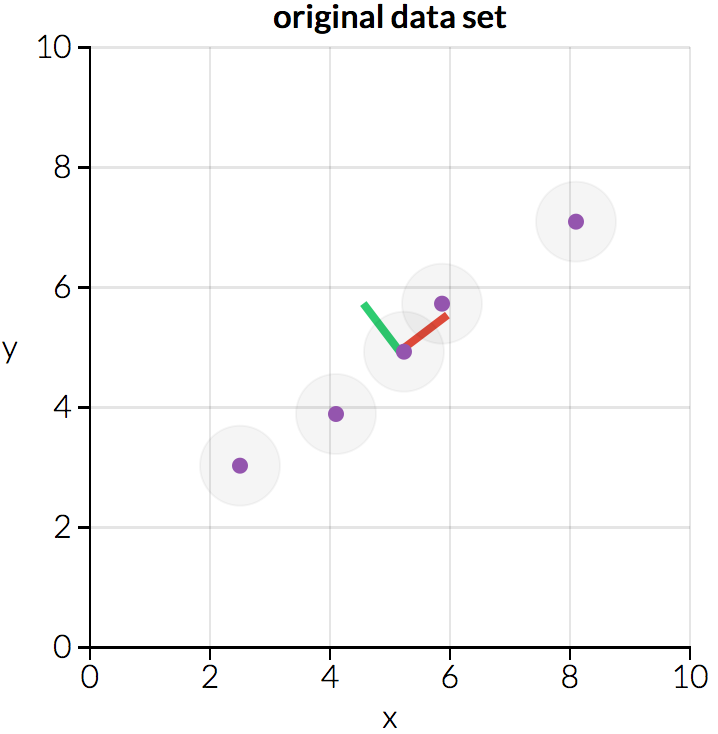
\includegraphics[width=0.45\textwidth]{Chapter-4/figs/pca_real_data}
    }
    \hfill
    \subfloat[Example: Data Projected on Eigen Plane\label{subfig:pca_proj_data}]{%
      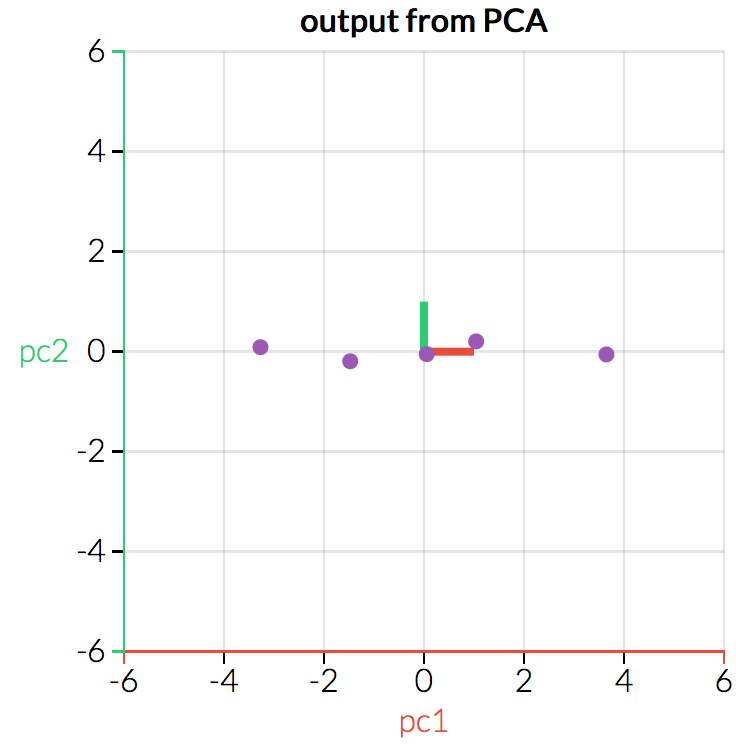
\includegraphics[width=0.45\textwidth]{Chapter-4/figs/pca_proj_data}
    }
    \caption{PCA Projection Example}\cite{pca_visual}
   \label{fig:pca_prog_eg}
 \end{figure}
  
  We can also see from figure \ref{subfig:pca_proj_data} that maximum variance of data is along the \textbf{pc1 axis}. This makes the \textbf{pc1 axis} the 1st principal component of the data. Using this property of PCA we can choose the most important \textit{features} only from a data set while excluding the less important \textit{features}. We see from \textbf{figure} \ref{pca_real_data_on_axis}, real data needs both the \textbf{x and y plane} to represent the features (spread) of the data. On the other hand in \textbf{figure} \ref{pca_proj_data_on_axis} we can see that most of the variance for the data items has been condensed with negligible variance along the \textbf{pc2 axis}. All features of the data can now be abstracted onto the \textbf{pc1} plane. This method is the method we use for data abstraction while maintaining the features of the data set.% \ref{fig:pca_feature_set_abstraction} \ref{pca_proj_data_on_axis} \ref{pca_real_data_on_axis}
 
 \begin{figure}[!ht]
	\centering
    \subfloat[Example: Variance for Real Data on X and Y axis individually\label{pca_real_data_on_axis}]{%
      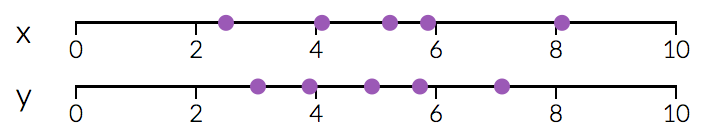
\includegraphics[width=0.45\textwidth]{Chapter-4/figs/pca_real_data_axis}
    }
    \hfill
    \subfloat[Example: Variance of Data on PCA axis individually\label{pca_proj_data_on_axis}]{%
      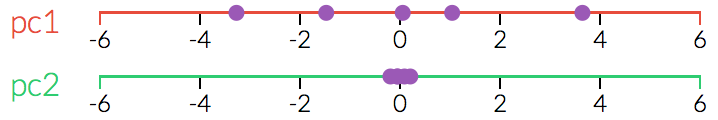
\includegraphics[width=0.45\textwidth]{Chapter-4/figs/pca_proj_data_axis}
    }
    \caption{Feature Set Abstraction}
   \label{fig:pca_feature_set_abstraction}
 \end{figure}
  
\subsection{Histogram Generation}
\label{hist_generation}
  Once the dimensionality of the data has been reduced using PCA, we need to reduce the point count ensuring we use the most dense distribution areas for data set comparisons. We tackle this problem by the use of Histograms.
Histogram is then generate on a per dimension \textit{(di)} basis with each dimension having 16 or 32 buckets with ranges computed as follows : 
\begin{equation}
     \begin{aligned}
       & bucket\_count = 16 \ or \  32 \\
       & dim\_bucket\_range_{di}\  =\  max_{di} \   - \   min_{di}: \  \forall\  di\  in\  (1\   ..\   3) \\
       & bucket\_size_{di} \   = \   dim\_bucket\_range_{di} \   / \    bucket\_count \ : \  \forall\  di\  in\  (1\   ..\   3) \\
       &  bucket\_range_j = [(bucket\_size * bucket_j + min_{di}), (bucketSize * (bucket_j + 1) + min_{di})); \\  
       & \forall \ j \ in \ (1\ .. \ n)
     \end{aligned}
\end{equation}

This will give us the buckets with their ranges for all dimensions. We then proceed to generate \textit{three} histograms. Each data point is put into a bucket based on its value for that particular dimension. 
\textit{E.g.:} let \textit{three points} be represented in a 3-D Eigen plane by coordinates as follows: \\
$p1 = (1,\ 2,\ 3)$
$p2 = (-1,\ 0,\ 1)$
$p3 = (2,\ 3,\ 4)$ \\ 
Now, let there exist 2 buckets per dimension with Ranges as follows:  \\
$b_{11} = [-1,\ 2)$
$b_{12} = [2,\ 4)$
$b_{21} = [0, \ 2)$
$b_{22} = [2, \ 4)$
$b_{31} = [1, \ 3)$
$b_{32} = [3, \ 5)$ \\

Using the above points and bucket ranges we will now generate \textbf{3 Histograms}(one per dimension) with \textbf{2 buckets per histogram.} The histograms may be represented as follows: \\
$h\_points_1\ =\ {b_{11}\ :\  (p1,\  p2);\ b_{12}\ :\  (p3)\ };\ \text{Histogram for first dimension}$\\
$h\_points_2\ =\ {b_{21}\ :\  (p2);\ b_{22}\ :\  (p1, \ p3)\ };\ \text{Histogram for second dimension}$\\
$h\_points_3\ =  {b_{31}\ :\  (p2);\ b_{32}\ :\  (p1, \ p3)\ };\ \text{Histogram for third dimension}$\\

Thus we can see from above example how each item becomes a part of a bucket if its coordinate for the given dimension lies in the bucket range for that dimension.

\subsection{Similarity Metric Computation}
\label{similarity_metric_calculation}
We now use the Welch's Test \cite{welch_test}\cite{boost_graph} to compute the probabilistic metric for similarity and to rank all history data sets wrt to each other and store in decreasing order of similarity. (Note: Will be used in run time historical reuse data set computation.) 
Welch test is computed for each dimension of the two sets being matched and the summation of the score for all three dimensions is as Similarity score for the two data set. Data sets are then ranked with each other based on the similarity score. Higher score means a better and match and vice versa.
\subsection{Training Algorithm}
This part of the algorithm is used to prepare and store data so as to have highest availability of reuse components for all candidates. We try and solve the challenges mentioned in \autoref{chap-three} using the methods mentioned in \ref{overview}. 
Let our history database consist of "n" data sets named: $HD_1, HD_2, ... HD_n$.
The following Steps are done for each $HD_i \text{  for (i in 1 to n) } $:
\begin{itemize}
    \item \label{pca_gen_training} \textbf{PCA:} Compute Eigen vectors for $HD_i$ and project data on the Eigen vectors to normalize in Eigen plane and reduce dimensionality as shown in \ref{principal_comp_analysis}. We reduce all data into 3-D space for comparison purposes.
    \item \label{his_gen_training} \textbf{Histogram Generation:} Categorize PCA data for $HD_i$ buckets for histograms as shown in \ref{hist_generation}. One histogram is generated per dimension of data, thus we have a total of 3 histograms for each data set. Each histogram comprises of a total of 32 buckets. 
    \item \textbf{Relative Ranking:} Use Welch Test to rank all history data sets wrt to each other. Data sets are stored in decreasing order of similarity as shown in Algorithm \ref{hist_relative_ranking}. (Note: Will be used in run time historical reuse data set computation.)
    \item \textbf{Reuse Data for Data Set:} Run Algorithm of choice for Data Set and store \textit{Computation Reuse Data}. E.g.: In case of the K-means algorithm we choose the \textit{final centroids} computed by the K-Means Algorithm for current data set.
\end{itemize}


%==================================================================
%			History Rank ALGORITHM	BEGIN
% ==================================================================
\begin{algorithm}
\caption{History Data Sets- Relative Ranking}
\label{hist_relative_ranking}
\begin{algorithmic}[1]
\Procedure{RankHistoryData}{$History\_Database$}
\State $relative\_rank_{map}\ =\ ORDERED\_MAP(Similarity\_Score,\ Data\_Set)$
\State $score_{Final} = 0$
\For{each $HD_i$ in $History\_Database$}
	\For{each $HD_j$ in $History\_Database$ != $HD_i$}
		\State $score_{Final}$ = $ComputeSimilarity(HD_i,\ HD_j)$
		\State $relative\_rank_{map}.insert(score_{Final},\ HD_j)$
	\EndFor
	\State$(HD_i).Relative\_Ranking$ = $relative\_rank_{map}$
\EndFor
\EndProcedure
\end{algorithmic}
\end{algorithm}

%==================================================================
%			History Rank ALGORITHM	BEGIN
% ==================================================================

%==================================================================
%			Welch ALGORITHM	BEGIN
% ==================================================================
\begin{algorithm}
\caption{Similarity Metric Computation}
\label{similarity_computation}
\fontsize{10}{15}
\begin{algorithmic}[1]
\Procedure{ComputeSimilarity}{$Data\_Set_{Current},\  Data\_Set_{Historic}$}
\State $score_{Final} = 0$
\State $Data_{CurDS} = TOP\_THREE\_BUCKET\_DATA(Data\_Set_{Current})$
\State $Data_{HistDS} = TOP\_THREE\_BUCKET\_DATA(Data\_Set_{Historic})$
\For{each $dim_i$ in $Dimensions(Data\_Set_{Current})$}
	\State $score_{Final}$ += $CalcWelchScr(Data_{CurDS}.columnAt(dim_i),\ Data_{HistDS}.columnAt(dim_i))$
\EndFor
\State\Return $score_{Final}$
\EndProcedure
\end{algorithmic}
\end{algorithm}

%==================================================================
%			SCREENING ALGORITHM	BEGIN
% ==================================================================

 
\begin{algorithm}
\caption{Screening Algorithm}
\label{screening_algo}
\begin{algorithmic}[1]
\Procedure{Screening\textendash PrimaryCandidateSelection}{}
\State $least\_distance_{rank} = MAX$
\State $least\_distance_{range} = MAX$
\State $dim\_distance_{rank} = 0$
\State $dim\_distance_{range} = 0$
\State $HD\_Rank_{selected}$
\State $HD\_Range_{selected}$
\For {each $HD_x$ in History Database} 
	\For { each $Dim_i\  where\ i\  in\  1\  ..\  3\ $ }
		\For{each  $Bucket_j$ in Top 3 Buckets($Dim_i$) in Decreasing Order of Item Count for current data set} 
			\State 
			\For{each  $pt_{cd}$ and $pt_{HDi}$ in points($Bucket_j$)} 
				\State $distance_{rank}\ =\  dist(pt_{cd},\ pt_{HDi})$;
			\EndFor

			\State$Bucket_k$ = Bucket in $HD_i\  where\ range(bucket_k)\ \sim \  range(bucket_j)$
			
 	 		\For {each  $pt_{cd}\  in\ points(Bucket_j)\ and\ pt_{HDi}\ in\ Bucket_k$ } 
				\State $distance_{range}\ =\ dist(pt_{cd},\ pt_{HDi})$;  
			\EndFor
		\EndFor
 	 		
		\State $dim\_distance_{rank}\  =\  dim\_distance_{rank} \ + \ distance_{rank}$
		\State $dim\_distance_{range}\  =\  dim\_distance_{range} \ + \ distance_{range}$ 
	\EndFor
	\If{$dim\_distance_{rank}$ < $least\_distance_{rank}$}
 			\State $least\_distance_{rank}$ = $dim\_distance_{rank}$;
			\State $HD\_Rank_{selected}\ = \ HD_x$;
	\EndIf
   	 
	\If{$dim\_distance_{range}$ < $least\_distance_{range}$}
   		\State $least\_distance_{range}\ = dim\_distance_{range}$;
   	 	\State $HD\_Range_{selected}\ = \ HD_x$;
	\EndIf
\EndFor
\State\Return [$HD\_Rank_{selected}$, $HD\_Range_{selected}$]
\EndProcedure
\end{algorithmic}
\end{algorithm}


%==================================================================
%			SCREENING ALGORITHM	END
% %================================================================

%==================================================================
%			Best Match Computation ALGORITHM	BEGIN
% ==================================================================
 
\begin{algorithm}
\caption{Best Match Selection Algorithm}
\label{best_match_selection}
\fontsize{10}{15}
\begin{algorithmic}[1]
\Procedure{BestMatchSelection}{}
\State $primary\_candidates = Screening$\textendash$PrimaryCandidateSelection$
\State $best\_match\_score_{final} = INT_MIN$
\State $best\_match\_score_{cur}$ = $ComputeSimilarity(Data\_Set_{current},\ primary\_candidates[0])$
\State $best\_match_{data\_set} = primary\_candidates[0]$
\State $best\_match\_score_{cur}= ComputeSimilarity(Data\_Set_{current},\ primary\_candidates[1])$
\If{$best\_match\_score_{cur}$ > $best\_match\_score_{final}$}
	\State $best\_match\_score_{final} = best\_match\_score_{cur}$
	\State $best\_match_{data\_set} = primary\_candidate[1]$
\EndIf
\For {each $HD_x$ in $TOP\_THREE{relative_rank}$($primary\_candidates[0]$)} 
	\State $best\_match\_score_{cur} = ComputeSimilarity(Data\_Set_{current},\ HD_x)$
	\If{$best\_match\_score_{current}$ > $best\_match\_score_{final}$}
		\State $best\_match\_score_{final} = best\_match\_score_{cur}$
		\State $best\_match_{data\_set} = HD_x$
	\EndIf
\EndFor

\For {each $HD_y$ in $TOP\_TWO_{relative_rank}$($primary\_candidates[1]$)} 
	\State $best\_match\_score_{cur} = ComputeSimilarity(Data\_Set_{current},\ HD_y)$
	\If{$best\_match\_score_{cur}$ > $best\_match\_score_{final}$}
		\State $best\_match\_score_{final} = best\_match\_score_{cur}$
		\State $best\_match_{data\_set} = HD_y$
	\EndIf
\EndFor
\Return  $best\_match_{data_set}$
\EndProcedure
\end{algorithmic}
\end{algorithm}

%==================================================================
%			Best Match Computation ALGORITHM	END
% %================================================================


\subsection{Computing Best Match for Current Data-set (Run Time)}
This is the part of the algorithm that is actually responsible for the selection of the 
\begin{itemize}
	\item \textbf{PCA:}  Compute PCA for current Data Set similar to \ref{pca_gen_training}.
	\item \textbf{Histogram Generation:} We again characterize PCA data into 3 histograms with 32 buckets each as done in \ref{his_gen_training}.
	\item \textbf{Matcher and Selector :}The best match data set selection process is divided into 2 parts: screening and final selection. Screening is used to prune our Historical Data Sets to a smaller subset from which we can select our best match Data Set for computation reuse using the final selection step.
	
	The two parts of the Matcher and Selector part of our algorithm may be defined as follows:
	\begin{itemize}
	\item \textbf{Screening:} This is the process where we select our initial candidates for the next step of our selection algorithm. This part of the algorithm essentially estimates the similarity in distribution for the current and corresponding historical data sets using the  Histograms generated in the previous steps. Variance Similarity is estimated as follows:			
		\begin{enumerate}
    			\item Take top-k most populated buckets for current data set and select corresponding top-k bins from all history data sets and top-k buckets with closest min and max to current data-set top-k bins.
		    \item Find ED for these data points between current data set and all historical data sets.
    			\item Choose Historical Data Sets with minimal distance as initial “Best Match” for both top-k buckets by rank and top-k buckets by range.
		\end{enumerate}
	Pseudo Code for an understanding of how our \textit{screening algorithm} runs can be seen in Algorithm \ref{screening_algo}.
	\item \textbf{Find Best Match (Similarity Metric => Probabilistic Score):} 
	One we have found the best match candidates from out screening step, we simple calculate the Welch Test score for each dimension ($dim_i$) for each pair of current data set and chosen historic data sets.
		\begin{enumerate}
    			\item Find ``Similarity Metric`` as expalined in subsection \ref{sim_calc} and between current data set and above chosen “best match” data sets using Welch’s Test for all dimensions of all three data sets as shown in Algorithm \ref{similarity_computation}.
		    \item Similarly find “Similarity Metric” for top two relatively ranked data sets for current best match and top one for second best match.
		    \item Choose Data Set with highest Probability Score.
		\end{enumerate}
			Pseudo Code for an understanding of how our \textit{final selection algorithm} runs can be seen in Algorithm \ref{screening_algo}.
	\end{itemize}		
	\item \textbf{Reuse Computations: }  In this section we use the computational data we had stored for history reuse in the training run for the historical data set selected. For instance, in the case of the K-Means algorithm, we now use the centroids from the chosen historical data set that were computed during the training run for historical data.
\end{itemize}
\section{Discussion}
Our final algorithm was reached at after a fair few trials and errors. Some of the major approaches used apart the latest approach for major challenges may be defined as below:
\subsection{Computation on Real Data and Incorrect Screening algorithm:}
\subsubsection{Implementation}
\begin{itemize}
    \item In this method I had initially use bin wise reduction on initial (real) data and then used PCA for dimension reduction of these reduced data points for the calculation of Eigen vectors and Eigen values only.
    \item I had then proceeded to run Student’s T-Test for relative ranking in training Run on real data.
    \item For Run Time computation I had used only the distance between the Eigen vectors for initial screening, choosing the data set with smallest difference in Eigen vectors as initial Best Match data set.
    \item I had then proceeded to Use Student T-Test on real data for computation of the probabilistic metric using all dimensions for the computation of the same.
    \item Python Numpy Libraries had been used for Student T-Test computation.
    \item History Reuse component Computations during training run was done on real data of historical data set instead of PCA data.
\end{itemize}
\subsubsection{Reasons for failure}
\begin{itemize}
    \item Data was not normalized thus computation would not be correct.
    \item Student T-Test worked only with Gaussian Distributions. Garbage value was returned for non Gaussian Data.
    \item Eigen Vectors of two data set may be orthogonal yet PDF (probability density function) may be close enough such as to generate similar clusters.
    \item Use of labels for direct initialization was flawed in the sense that if the data points were jumbled they would produce the wrong order of labels thus still providing a bad match.
    \item Bin Wise distribution of data points was an expensive operation and computation overhead increased with increase in dimensionality of data.
    \item Student T-Test had to compute for multiple dimensions of data and was a time expensive computation.
\end{itemize}
\subsection{Custom CPP Implementation for Welch’s Test}
Some of the earlier seen issues were corrected in this section as I noticed that a lot of the run time improvement was overshadowed by the time taken for choosing the historical data set. I also noticed that the Student T-Test was not reliable for non-Gaussian data and failed completely in case of different data set sizes.
This iteration was also mainly about ensuring quicker run time for the selection algorithm, so incremental updates were made to optimize the same. Some of the updates made may be enlisted as follows:
\begin{itemize}
    \item Implemented Custom Cpp implementation for Welch’s Test to over come overhead created by using python libraries for it and calling python script from Cpp.
    \item Removed the distribution of data into bins for data point reduction as it had a big overhead in computation and CPP Welch Test Libraries scaled well for larger data sets.
    \item Changed to use of Welch’s Test as compared to Student T-Test as Welch’s Test works with non Gaussian distributed data as well as compared to Student T-Test which makes assumptions of data distribution being Gaussian in nature.
    \item For Run Time computation I had used only the distance between the Eigen vectors for initial screening, choosing the data set with smallest difference in Eigen vectors as initial Best Match data set.
    \item Centroid Computation during training run was done on real data of historical data set instead of PCA data.
    \item Labels for Best Match historic data set were used as-is for current data set.
\end{itemize}
\subsection{Random Sampling for Order comparison.}
Experimentation on the approach showed non-reliable best match selection. Also I saw that often the best match might not even yield best results. One of the major reasons for this was the use of the incorrect use of historical data. For instance, in case of the K-Means algorithm the use of labels instead of the computed centroids lead to dependence on the order of the items in the historic data set. While the two data set may be similar and produce similar clusters, History Reuse with this method would still fail as initially the data points in current data set may get labeled incorrectly. I also realized that comparison of non-normalized data was in its very essence. I tried to correct the above issues with the following methodology:
\begin{itemize}
    \item Changed implementation to use of PCA data for most computations.
    \item Projected Historical data set points on Current Data Set Eigen Vectors. Used distance between data points of Current Data Set and historical data sets by randomly sampling 10\% of data sets against each other. Chose Data Set with minimum distance. This was done to try to use Historical data set with most point order similarity (and thus generated label order similarity) in conjunction with overall data set similarity.
    \item Welch’s Test was still used across all dimensions of actual data Similarity Metric Computation.
    \item Labels were used as-is for real data.
\end{itemize}
This implementation though corrected some of the above mentioned issues, it in its turn generated new issues:
\begin{itemize}
    \item Use of labels for direct initialization was flawed in the sense that if the data points were jumbled they would produce the wrong order of labels thus still providing a bad match.
    \item Random Sampling was a bad way to judge the order of the labels that would be generated by K-Means for data set.
    \item Eigen Vectors of two data set may be orthogonal yet PDF may be close enough such as to generate similar clusters.
\end{itemize}
\subsection{Use Of PCA Data for Welch’s Test and PCA data for centroid computation in Training Run:}
Experimentation still showed both the history reuse to be inconsistent and the overhead of computing historical data set was still quite large. I also realized that while Eigen Vectors of two data set may be orthogonal yet PDF might be close enough such as to generate similar clusters. To correct the above issues I used the following methods:
\begin{itemize}
    \item Used PCA data in training run for Centroid computation of historical data.
    \item Used PCA data for Welch’s Test based “Similarity Metric” computation.
    \item Still used labels from best match historical data set as initialization for current data set.
    \item Stopped projecting historical data sets data on current data set Eigen vectors, instead used self-projection, which could be done offline.
    \item Used Random Sampling for initial estimation of best match data set.
\end{itemize}
The use of Labels was still flawed. Also the use of random sampling was not a very effective methodology for screening as it would often lead to the selection of bad candidates.


